% Evidence-constrained working draft. This is NOT the unavailable supplied manuscript.
% Compile with: pdflatex manuscript.tex; pdflatex manuscript.tex
\documentclass[11pt]{article}
\usepackage[T1]{fontenc}
\usepackage[margin=22mm]{geometry}
\usepackage{graphicx,booktabs,longtable,hyperref}
\title{A reproducible structure-to-XAS workflow for adsorbate inference at Cu--Au interfaces}
\author{[Author list and affiliations to be confirmed]}
\date{Evidence reconciliation: 21 October 2026}
\begin{document}
\maketitle
\begin{abstract}
We connect generated catalytic structures, relaxation inputs, simulated X-ray absorption spectra, ISAAC records, and grouped adsorbate-presence inference. The completed Cu K-edge benchmark contains 87 independent configurations with four available layer spectra per configuration. Frozen configuration-level outer folds yield micro/macro F1 of 0.7791/0.6383 for the primary independent-species selector, with exact identity-set accuracy 0.6897. The highest observed fixed-entry result, 0.7978/0.6597, was selected after examining outer scores and is exploratory. Portable byte-hashed cohort export, read-only connectivity and population audits, and saved-model replay reproduce these results without changing measurement arrays. Matched coupled/uncoupled comparisons, numerical experimental references, robustness on a new confirmation set, execution-rate estimates, and portal deposition remain unmeasured or unavailable. This working draft follows the accessible two-page outline; the named supplied manuscript and its provenance package were unavailable during reconciliation.
\end{abstract}

\section{Introduction}
Adsorbate identification from metal-edge XAS requires accounting for the substrate, adsorption environment, surface sensitivity, and the distinction between multiple adsorbates and bonded intermediates. A reproducible workflow must preserve the relationship between requested chemistry and observed relaxed connectivity, document which absorbers contribute to each spectrum, and prevent related spectra from leaking across evaluation folds. Here we report completed identity/depth results and distinguish them from the broader study plan.

\section{Methods and implementation}
\subsection{Workflow and authorization boundary}
The implementation includes structure generation, periodic contact checks, relaxation/XAS preparation, restartable execution helpers, record conversion, and inference (Figure~\ref{fig:framework}). Preparation and local replay are not evidence of autonomous execution success. HPC submissions, external record deposition, and branch merging were not performed in this reconciliation. Parallel generation/orchestration routes remain separate; regression tests exercise their existing relaxed-geometry and label behavior.

\subsection{Inventory and chemical labels}
The source inventory contains 172 locations and 155 unique structures, including unfinished structures and a CuO reference. The 102 completed-record files reduce to 87 independent configurations after 14 duplicates and one incompatible-grid record are removed. Molecular species are positive binary outputs; CO+H and CO+OH are coadsorption sets, while COCHO and OCCOH are distinct bonded intermediates. There are 78 single-species and nine mixed configurations: five CO+H, three CHO+CO+H, and one CO+OH. Species supports overlap and sum to 99. No eligible clean control or intact OCCO positive is available.

The new read-only component audit uses actual XAS input coordinates, mapped atom membership when available, and disclosed connectivity cutoffs for legacy structures. It uses exact in-plane minimum images with a nonperiodic vacuum, rather than rounding all fractional coordinates. A $\pm10\%$ cutoff sensitivity check preserves ambiguous cases for review. The seven corrected component/count examples reproduce their current labels. Their measurement arrays are unchanged. The layer-specific converter identified in record provenance is absent from the repository and accessible local converter files; its actual producer cannot be repaired by assuming that the general root converter owns that code.

\subsection{Spectral populations and depths}
Available Cu layers are 2--5; layer 5 is the physical top. Final convolution evidence supersedes subset-recalculation main decks and intermediate logs. The two recovered CO configurations have 36-site final convolutions. Site-file coverage, Cu elements, heights, compatible grids, and site-to-log $E_{\mathrm{cut}}$ agreement are checked, preserving the approximately 0.00051 eV log-rounding tolerance. Original source symmetry multiplicities are retained as evidence; population counts refer to unique physical layer Cu indices. Compatible raw layer spectra are population weighted before normalization. The four-layer average represents four available layers, not the entire five-layer slab or an experimental bulk measurement.

\subsection{Grouped inference and saved-model replay}
The archived protocol compares normalized shape, cumulative distribution functions, derivatives, combined shape/CDF/derivatives, DCT24, and additional tree depth/multiscale representations using logistic regression, RBF SVM, random forests, joint extra-trees, and independent species extra-trees. All layers and variants of a physical configuration remain in the same frozen outer fold. Learned preprocessing, model selection and thresholds use training data only. The general application's categorical advisor is separate from this multilabel benchmark. A new explicit multilabel route uses shared audited loading, spectral recipes, binary outputs and training-only selection.

Archived truth/prediction arrays are replayed before fitting. All five primary models, refitted with their archived training-selected recipes and thresholds, reproduce the held-out predictions exactly after serialization/import from a relocated cohort export. A fold with no positive COCHO training examples is reported. Training-only majority-binary and most-common-identity-set constant baselines use the same outer folds. This repeatedly examined cohort is not independent confirmation of newly selected workflows. Conditional bootstrap intervals on saved OOF predictions are not confidence intervals from model retraining.

\section{Completed results and bounded interpretation}
\subsection{Inventory and depth dependence}
Figure~\ref{fig:inventory} separates the planned structural matrix from actual completion. Pure Cu(111)/Au(111), stripe ratios 1:1, 2:1, 1:2 and 6:2, interface/near-interface/terrace sites, coverage/distribution controls, and C1/C2/coadsorbate states remain a design matrix rather than an assertion that every cell exists. The matrix file records explicit minimum row counts and inferred source-ratio matches; region completeness is not inferred from names.

The primary selector yields micro/macro F1 0.7790697674/0.6382765883 and exact set accuracy 0.6896551724 (Figure~\ref{fig:inference}). Fixed-depth nested selection yields 0.7861271676/0.6428295066 for the top layer, 0.7444444444/0.6253068197 for the top two, and 0.6593406593/0.5082757013 for four available layers. These point estimates favor the top layer on this cohort; paired conditional uncertainty is reported separately. The exploratory best fixed entry uses top-layer first derivatives and extra-trees, with micro/macro F1 0.7978142077/0.6597402597 and exact set accuracy 0.7011494253. It must not be promoted to independent validation.

CO2, COCHO and OCCOH supports are only 3, 1 and 4, respectively. Mixture recall and per-species confusion tables distinguish omissions from wrong-species positives. Independent clean controls, rare species and matched CO/CO+H/CO+OH configurations have higher priority than extra layers or site spectra of existing structures. Exact additional sample counts should be designed around chemical balance and feasible confirmation holdouts, not apparent dataset size.

\subsection{References and complementary edges}
Figure~\ref{fig:spectra} contains real normalized layer spectra and explicit unfinished panels. Numerical Cu/Cu2O/CuO reference metrics require raw traces, source/license, backend version and mode, structure, core-hole treatment, convergence, broadening, energy calibration, fitting interval and allowed alignment parameters. The named CuO benchmark PDF was unavailable; an image alone would not support exact metrics in any case. The reference-comparison utility records unshifted and permitted aligned normalized RMSE, Pearson correlation and edge/peak displacements, and rejects extrapolation and plot-derived precision claims. C/O generator probes are implementation evidence, not completed or converged complementary-edge results.

\subsection{Matched coupling test}
The repository's four input structures share a cell and metal parent and each contain two C and two O atoms (Figure~\ref{fig:matched}). Minimum input C--C distances are approximately 2.52, 2.46, 1.45 and 1.45 \AA. The loading is 2/36 C equivalents per top-layer Cu site; one OCCO and two CO have different molecular coverage. Final trajectories are linked by initial-geometry hashes rather than folder names. No verified completed matched Cu/C/O coupling contrast or independent coupling-state classifier is reported. Missing-job manifests are preparation only. Dissociated relaxed OCCO must remain dissociated evidence, not a coupled positive. Spectral contrast alone cannot establish an activation barrier or selectivity.

\subsection{Execution and record reuse}
Surviving scheduler stdout supports 735 surviving stdout files corresponding to 651 distinct scheduler job IDs across 93 canonical workflow folders, not a reconciled attempted-run denominator. Scheduler terminal state, process exit code, numerical validity, record creation, and ML eligibility are distinct fields. Missing accounting, restart intent and manual-action histories prevent first-pass/recovery success, retry-cost and intervention-rate estimates. Local fixture round trips test stable IDs, unchanged measurement/identity hashes, and prediction identity; they are not portal receipts or deposition/reuse results.

\section{Discussion and remaining work}
The result connects a concrete Cu K-edge identity task to a traceable structure/record pipeline. It does not establish geometry, coverage, C/O edge, coupling, robustness, calibration, or out-of-distribution performance. Geometry/coverage supports are exported separately and prediction performance remains unmeasured. A genuinely new confirmation set must be frozen before selecting perturbation ranges grounded in the intended experiment and evaluating shifts, noise, broadening or augmentation. One-parent holdouts may be infeasible and should be stated rather than presented as independent-parent validation.

\section{Conclusions}
A frozen 87-configuration multilabel benchmark is reproducible from archived OOF artifacts and from a relocated exact-cohort export with saved-model replay. Shared audits and explicit task separation improve implementation consistency while preserving the established scientific result. Unmeasured analyses remain identified as planned work.

\begin{table}[ht]\centering\small
\caption{Inventory, labels and coverage. Counts refer to independent structures unless specified.}\label{tab:inventory}
\begin{tabular}{lr}\toprule Item & Count/status\\\midrule
Source locations / unique inventory & 172 / 155\\
Completed records / duplicates / incompatible-grid case & 102 / 14 / 1\\
Eligible configurations / layer spectra & 87 / 348\\
Single / mixed configurations & 78 / 9\\
Overlapping species positives & 99\\
Clean controls / intact OCCO eligible positives & 0 / 0\\
Rare CO2 / COCHO / OCCOH positives & 3 / 1 / 4\\
Quartet C-equivalent loading & 2 / 36 top-layer Cu sites\\\bottomrule
\end{tabular}\end{table}
\begin{table}[ht]\centering\small
\caption{Backend/edge evidence and reference status. Generator success is not numerical validation.}\label{tab:backend}
\begin{tabular}{lll}\toprule Backend & Evidence & Numerical reference metrics\\\midrule
FDMNES, Cu K & completed audited cohort & experimental RMSE/r unmeasured\\
FDMNES, C/O K & generated input probes & raw outputs unavailable\\
FEFF, C/O K & generated input probes & raw outputs unavailable\\
VASP, C/O K & generator compatibility tested & raw outputs unavailable\\
Cu/Cu2O/CuO experimental comparison & protocol implemented & provenance/raw traces unavailable\\\bottomrule
\end{tabular}\end{table}
\begin{table}[ht]\centering\small
\caption{Workflow evidence. Missing denominators prevent execution-rate claims.}\label{tab:execution}
\begin{tabular}{ll}\toprule Quantity & Evidence/status\\\midrule
Surviving stdout files / distinct job IDs & 735 / 651\\
Canonical observed workflow folders & 93\\
Reconciled attempted-run denominator & unavailable\\
Scheduler success vs numerical validity & separated, not interchangeable\\
First-pass/recovery success rates & unmeasured\\
Retry cost / manual intervention rates & unmeasured\\
Record deposition / retrieval receipts & unavailable; local fixtures only\\\bottomrule
\end{tabular}\end{table}

\clearpage
\begin{figure}[p]\centering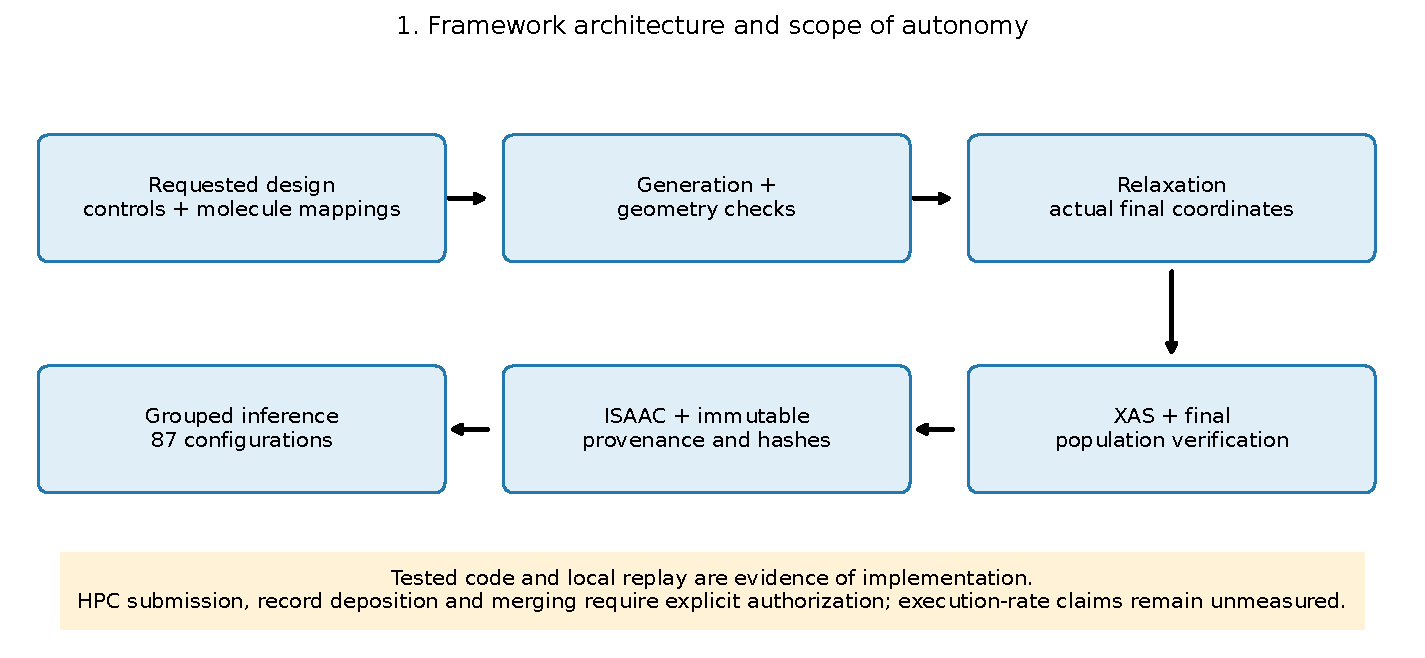
\includegraphics[width=\textwidth]{figures/figure_1_framework.pdf}\caption{Framework architecture and scope of autonomy. Requested design, generation, relaxation, XAS population verification, records and grouped inference are connected by traceable artifacts. Implementation/replay evidence is distinguished from authorization to submit jobs or publish records.}\label{fig:framework}\end{figure}
\begin{figure}[p]\centering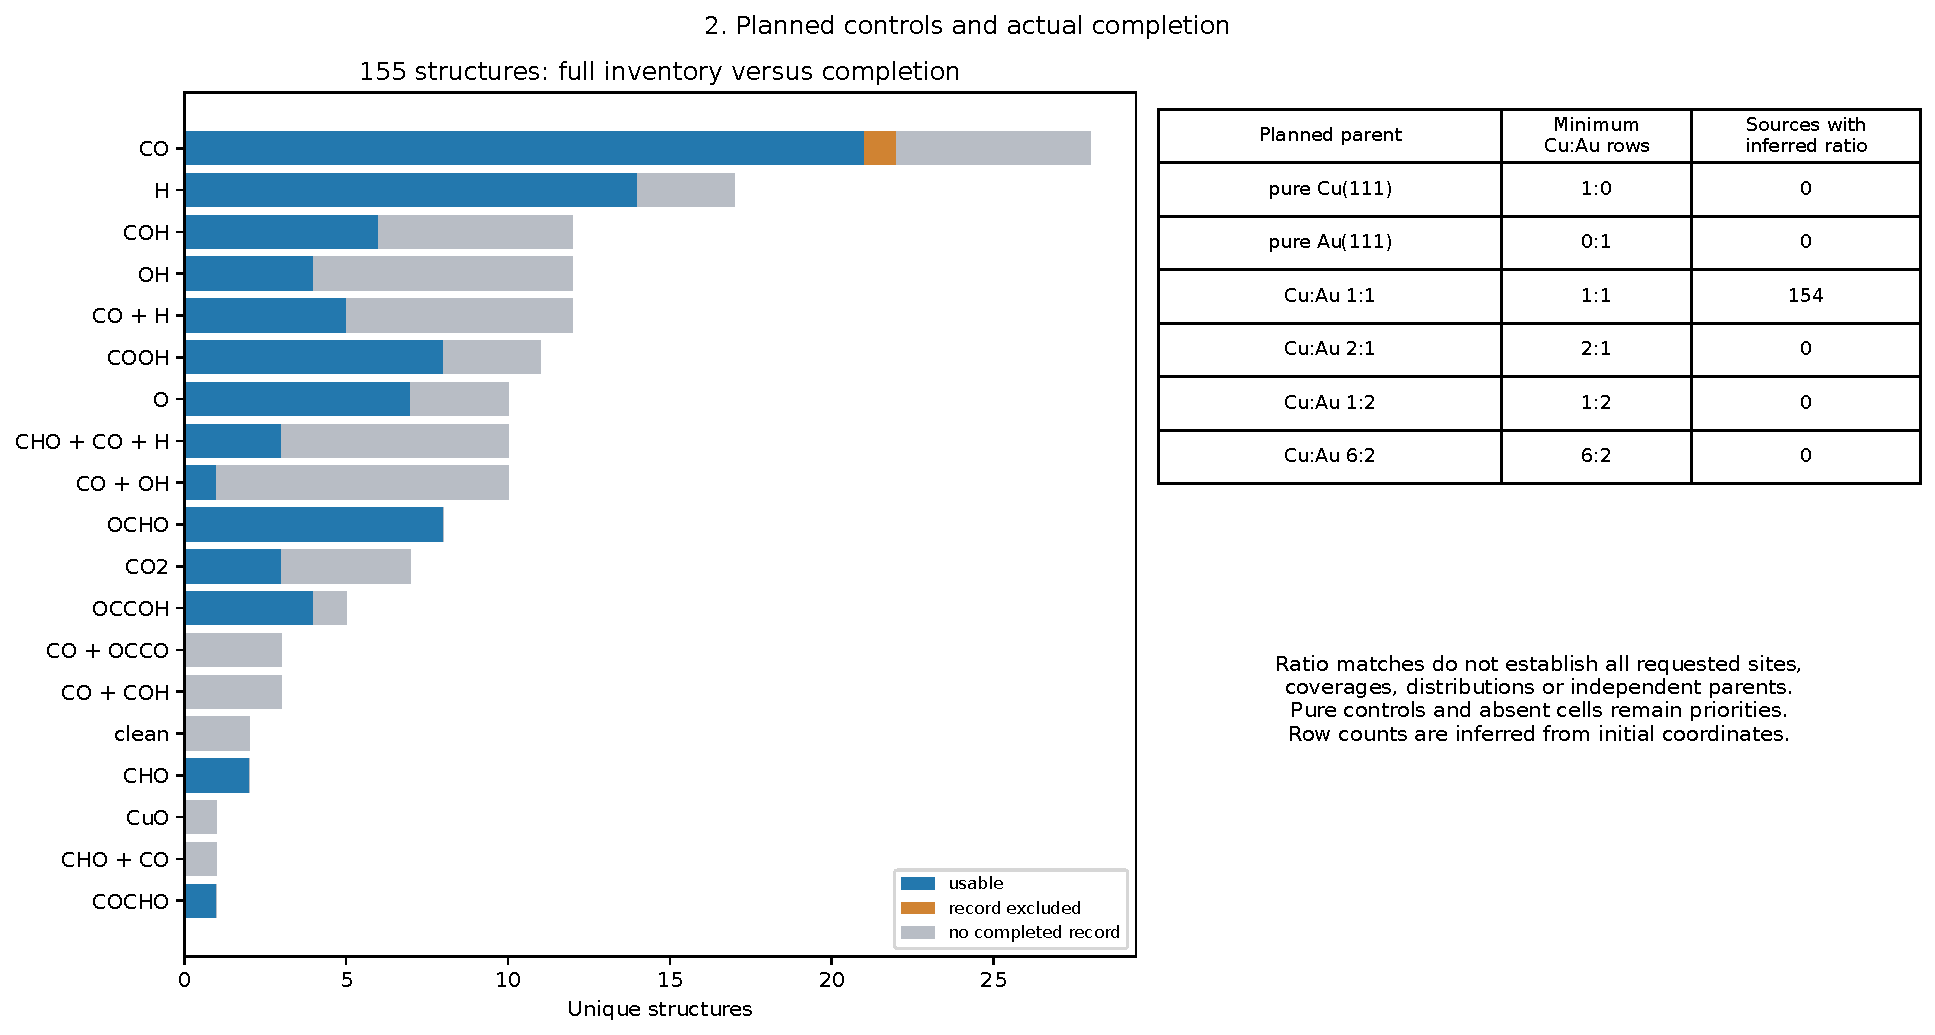
\includegraphics[width=\textwidth]{figures/figure_2_inventory.pdf}\caption{Planned controls versus completion. The full unique inventory includes unfinished structures and CuO. Parent row ratios and source matches do not demonstrate that the complete site/coverage/distribution matrix exists. Mixture categories are exclusive combinations.}\label{fig:inventory}\end{figure}
\begin{figure}[p]\centering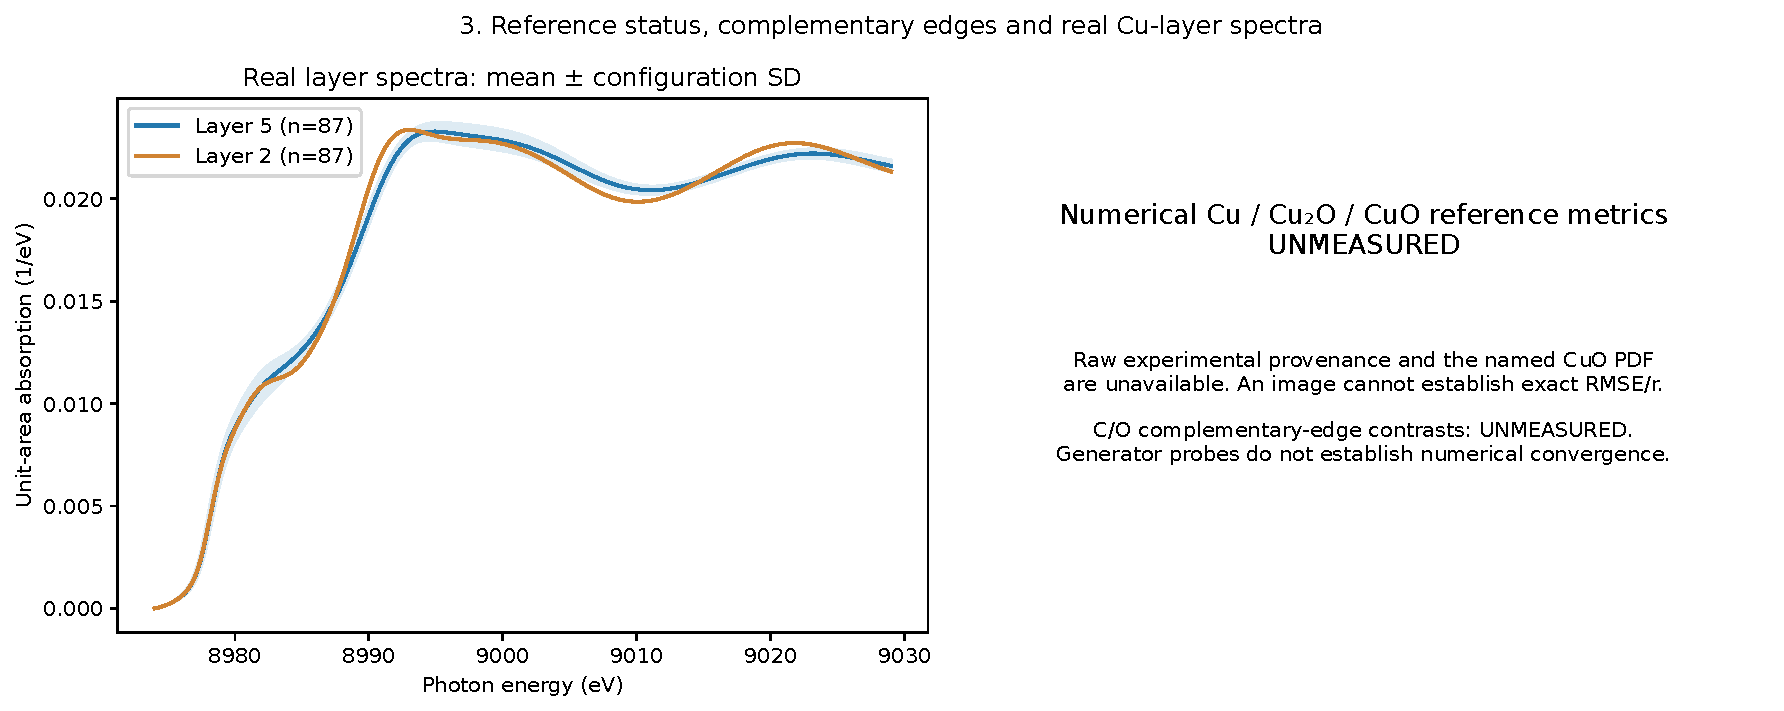
\includegraphics[width=\textwidth]{figures/figure_3_spectra.pdf}\caption{Real layer spectra and unfinished reference/complementary-edge analyses. Mean normalized absorption and configuration standard deviation are shown for layers 5 and 2 across 87 configurations. Shading is configuration variability, not a confidence interval. Numerical references and C/O contrasts remain explicitly unmeasured.}\label{fig:spectra}\end{figure}
\begin{figure}[p]\centering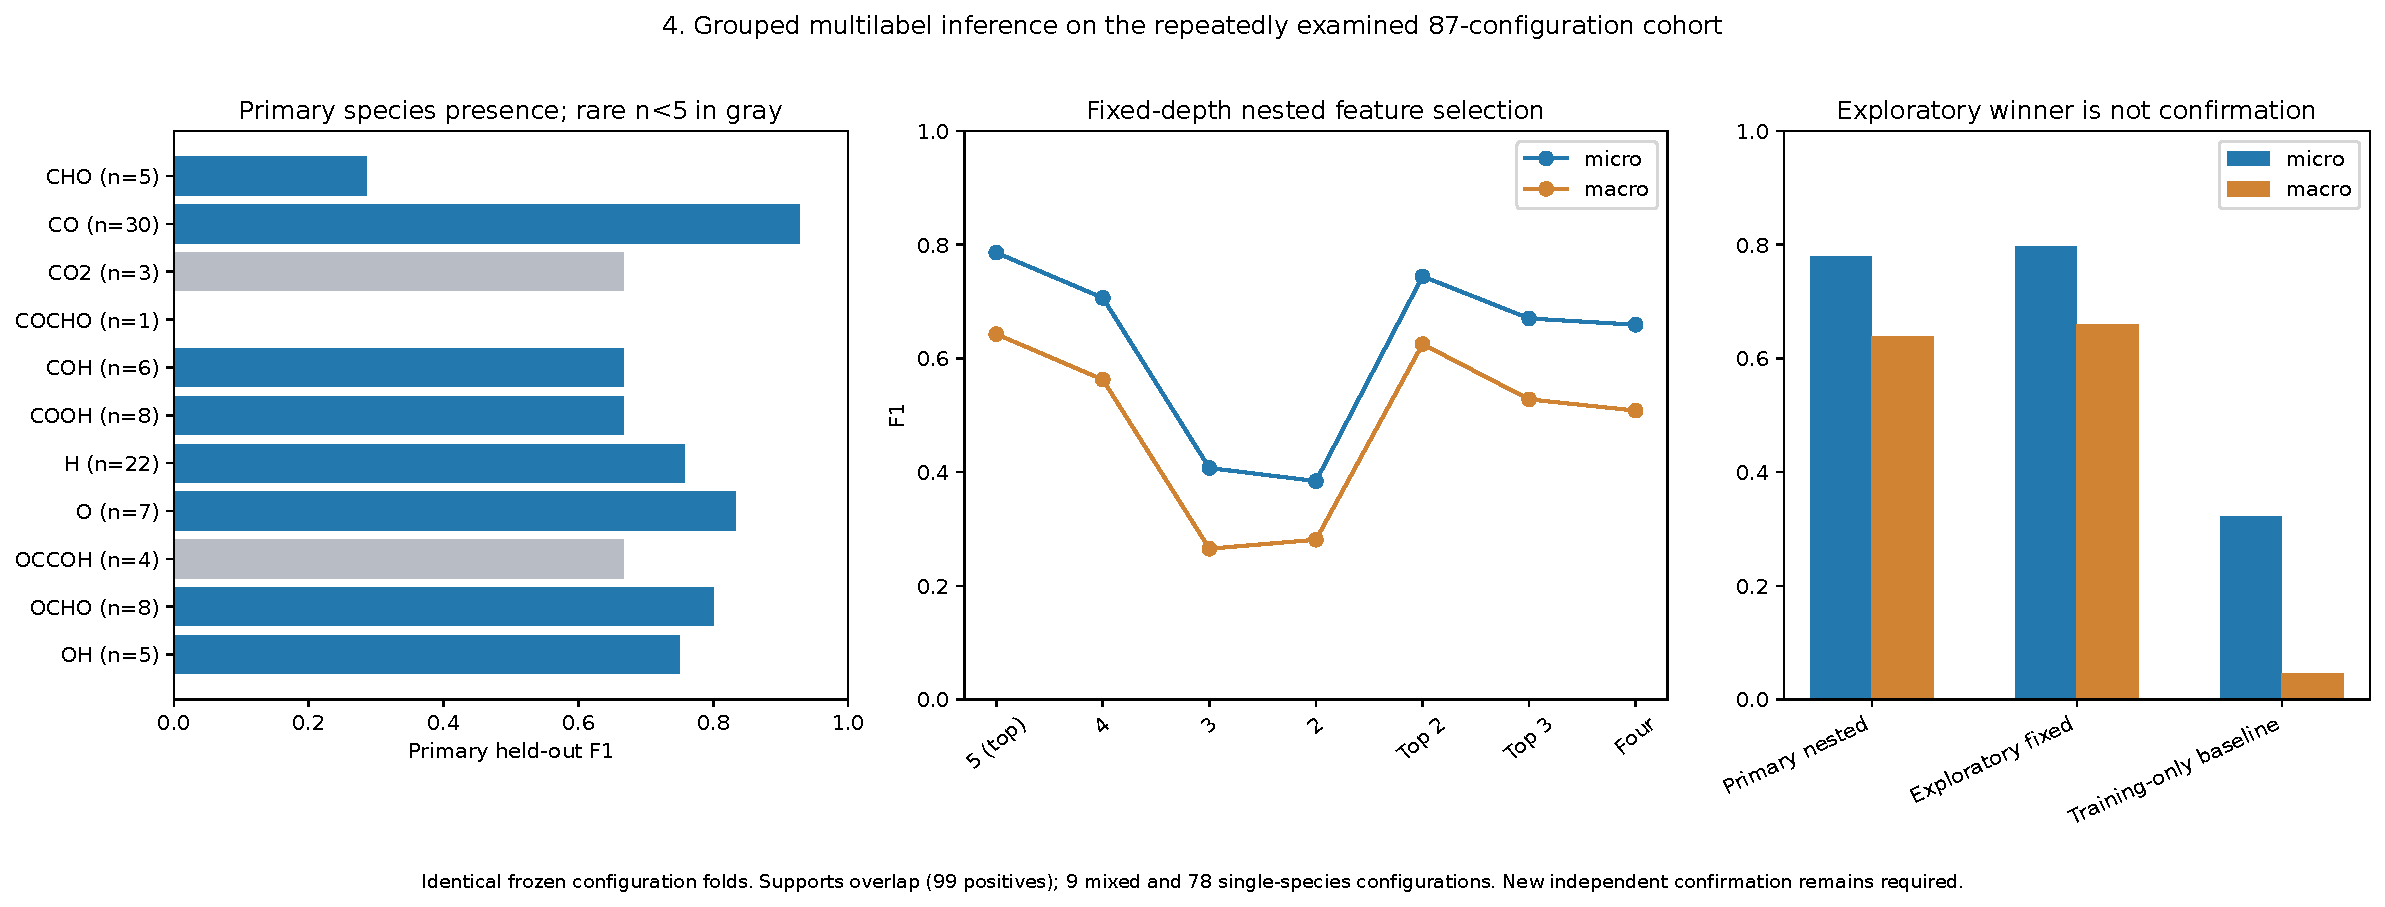
\includegraphics[width=\textwidth]{figures/figure_4_inference.pdf}\caption{Grouped adsorbate-presence inference. Per-species F1 and overlapping supports use the primary nested-selector OOF predictions. The depth panel uses fixed-depth nested feature/threshold selection. Aggregate primary, exploratory fixed-entry and training-only most-common-set baseline scores are distinct. Rare supports, repeated cohort use, and absent clean controls limit inference.}\label{fig:inference}\end{figure}
\begin{figure}[p]\centering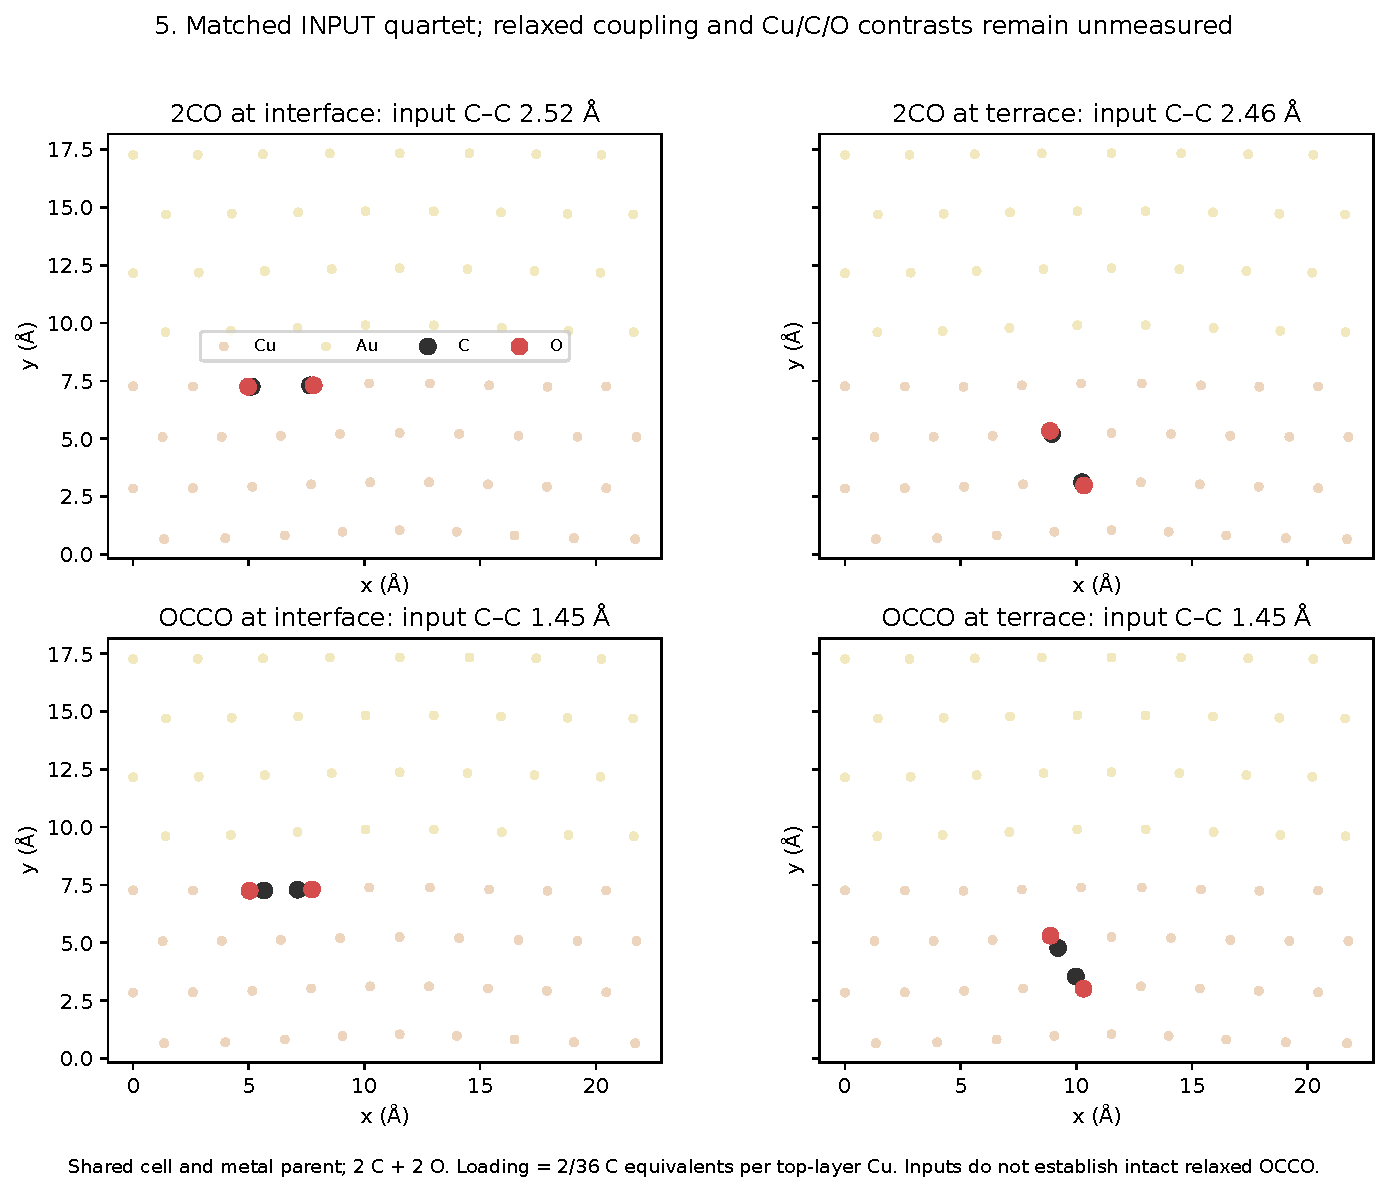
\includegraphics[width=\textwidth]{figures/figure_5_matched_inputs.pdf}\caption{Matched input quartet for two CO versus OCCO at interface and terrace sites. These are input coordinates, not completed relaxed coupling evidence. Shared loading is two C plus two O with 36 top-layer Cu sites; one OCCO and two CO differ in molecular coverage. Matched relaxed Cu/C/O spectra, population-dependent contrasts and interface-minus-terrace coupling contrast remain unmeasured.}\label{fig:matched}\end{figure}

\clearpage
\section*{Author contributions}
[To be confirmed by authors.]
\section*{Conflicts of interest}
[To be confirmed by authors.]
\section*{Data availability}
[Raw-data DOI to be confirmed.] The reviewed implementation and archived OOF artifacts are associated with repository commit \texttt{71bb0a2}. A local byte-hashed exact-cohort export has been prepared but not published. Full reproduction requires that export; figure-only replay uses committed plotted data and OOF arrays.
\section*{Acknowledgements and funding}
[To be confirmed by authors.]
\section*{AI disclosure}
[To be confirmed by authors.]
\section*{Source-package and template status}
This is an evidence-constrained working draft, not an overwrite or claimed reconstruction of the unavailable supplied manuscript. The accessible \texttt{CO2RR\_Agent\_Digital\_Discovery\_Outline.tex} supplies figure/table roles only. No file labelled as an RSC template was treated as a template. The named manuscript, original figure provenance/captions and CuO reference PDF are required for final editorial reconciliation.
\end{document}
